\documentclass[11pt]{article}

\usepackage[margin=1in]{geometry}
\usepackage{amsmath}
\usepackage{fontspec}
\usepackage{unicode-math}
\usepackage{microtype}
\usepackage{parskip}
\usepackage{booktabs}
\usepackage{array}
\usepackage{graphicx}
\usepackage{placeins}
\setlength{\emergencystretch}{3em}

% Map math symbols that the text font lacks to math-mode equivalents.
\usepackage{newunicodechar}
\newunicodechar{→}{\ensuremath{\rightarrow}}
\newunicodechar{←}{\ensuremath{\leftarrow}}
\newunicodechar{≤}{\ensuremath{\leq}}
\newunicodechar{≥}{\ensuremath{\geq}}
\newunicodechar{≈}{\ensuremath{\approx}}
\newunicodechar{−}{\ensuremath{-}}
\newunicodechar{×}{\ensuremath{\times}}
\newunicodechar{≠}{\ensuremath{\neq}}


\providecommand{\tightlist}{%
  \setlength{\itemsep}{0pt}\setlength{\parskip}{0pt}}

\usepackage{natbib}
\setlength{\bibsep}{2pt plus 0.3ex}

\usepackage{xcolor}
\definecolor{citecol}{HTML}{1A4D8F}
\usepackage[colorlinks=true,citecolor=citecol,linkcolor=citecol,urlcolor=citecol]{hyperref}
\usepackage[nameinlink]{cleveref}
\crefname{section}{section}{sections}
\Crefname{section}{Section}{Sections}
\crefname{table}{Table}{Tables}
\Crefname{table}{Table}{Tables}
\crefname{figure}{Figure}{Figures}
\Crefname{figure}{Figure}{Figures}

% ------------------------------------------------------------------
% JaleesBench-Mini — companion paper to JaleesBench (experiment 24).
% Status: DRAFT (2026-09-09). Every number comes from
% jaleesbench/results/mini_stats.json and mini_explore.json, produced by
% `python -m jaleesbench.mini run` / `explore` (seed 20260909).
% Prospective test (V4) run 2026-09-10 on IFM K2-Horizon-375B-A23B:
% results/mini_v4_k2-horizon.json (produced by `python -m jaleesbench.mini score`).
% ------------------------------------------------------------------

\title{JaleesBench-Mini: A Preregistered Item-Reduction Study\\
in Which Optimization Did Not Beat Sampling}
\author{
  M. Waleed Kadous\\[2pt] {\small iaser.ai \& Faith Family Technology Network}
}
\date{}

\begin{document}

\maketitle

\begin{abstract}
JaleesBench scores an AI assistant as a companion on 140 scenarios, each run
under six pressures, three framings and two judges; a full run costs on the
order of \$150 per subject plus judging. We ask how many scenarios a fixed
subset needs before it reproduces not just the headline score but the full
suite of reported quantities --- headline, ranking and sign, steadfastness
under pressure, and the stated/guided framing staircase --- for a subject it
has never seen. The study was preregistered: a 0.05 tolerance on every
quantity, leave-one-subject-out validation as the reported number, and two
hypotheses (a constrained greedy subset of at most 70 scenarios passes; random
subsets of that size mostly do not). Both hypotheses were falsified. The first
size at which greedy selection passes held-out is $k=110$ of 140, a 21\%
saving, and at that size 72\% of random subsets pass too. The reason is
arithmetic: a subject's per-scenario scores have a standard deviation near
0.5 on the $-1$ to $+1$ scale, so any $k$-subset carries a sampling error of
about $0.5\sqrt{1/k-1/140}$, and keeping the worst of some forty held-out
quantities under 0.05 needs $k\approx110$ whatever the selection method.
Greedy, annealing and a time-limited MILP all fit the training subjects
better (worst in-sample error 0.018, 0.012, and a 0.007 incumbent) with no
held-out benefit. The
110-scenario mini passes every never-in-selection check we had on hand ---
the Arabic replication (worst error 0.034, rank correlation 0.83 preserved)
and four follow-up model variants (0.024) --- and a prospective test on a
thirteenth subject released after the freeze, IFM K2-Horizon-375B-A23B,
passes with a worst error of 0.019. The mini is released frozen against
probe-bank v4 as a screening instrument. The full bench remains the citable
number. We argue that the sampling floor should be step zero of any benchmark
item-reduction study.
\end{abstract}

\section{Introduction}\label{sec:intro}

This paper reports a single, preregistered experiment on how far a behavioral
benchmark can be shrunk before it stops reproducing itself, and what the
result says about the item-reduction methods now common in language-model
evaluation. It is a companion to the JaleesBench paper \citep{jaleesbench2026},
which introduced the benchmark whose reduction is studied here.

JaleesBench measures whether an AI assistant is a \emph{jal\={\i}s
\d{s}\={a}li\d{h}} --- a righteous companion --- across 140 everyday
scenarios drawn from the chapters of \emph{Riy\={a}\d{d} a\d{s}-\d{S}\={a}li\d{h}\={\i}n}
\citep{nawawi-riyad}. Each scenario is a multi-turn sitting: an opening
request, then a pressure turn in which the user pushes toward the worse
course (secularizing, insisting, citing a false authority, invoking a good
cause, flattering, or appealing personally). Each sitting is run in three
framings (faith unstated, faith stated, and stated plus a one-page guide) and
judged by two frontier models on a five-band scale at two scopes, the first
reply and the full conversation. A subject therefore costs
$140\times6\times3$ sittings and twice that many judgments. The benchmark's
scorecard is a single number per subject, but the paper's findings rest on a
suite of quantities: the headline score, the ordering of subjects, how much
each subject gives way under pressure, and how much each gains from being
told the user is Muslim or from being handed the guide.

The obvious economy is a fixed subset of scenarios. A pilot analysis on the
existing judgments suggested it would be dramatic: a greedy 30-scenario
subset reproduced the headline score of each held-out subject to within
0.075. But that subset, selected on the headline alone, distorted
steadfastness by up to 0.13 and the framing scores by about 0.10. A mini that
reproduces the number on the scorecard while misreporting the findings behind
it is worse than no mini. So the question was re-posed with discipline:
fix the full suite of quantities, fix the tolerance, fix the validation, and
write down what would count as failure before running anything.

The answer is negative on the hypotheses and positive on the instrument. No
subset below 110 scenarios meets a 0.05 tolerance on every quantity for a
held-out subject, and at 110 the optimized subset is no better than a random
one. The mechanism is not subtle, and \cref{sec:floor} gives it in one line.
The 110-scenario subset itself is sound: it passes every out-of-sample check
we had, including a prospective test on a model released after the freeze,
and we release it frozen. The contribution of the paper is as much
the negative methodological result as the artifact: on a benchmark of this
shape, item selection cannot beat the sampling floor, and the floor can be
computed before any selection is attempted.

\section{Related work}\label{sec:related}

Reducing benchmark size is an active line of work, with approaches ranging
from psychometric item models to correlation-based anchor selection to
reliability accounting for benchmark design decisions. We describe the main
threads on their own terms.

\citet{polo2024tinybenchmarks} fit item-response-theory models to existing
evaluation results and show that about a hundred curated examples suffice to
estimate a model's MMLU accuracy to within a couple of points, releasing
tiny versions of several standard benchmarks. \citet{vivek2024anchor} observe
that model confidence on pairs of examples is strongly correlated across
models, and select small ``anchor point'' subsets that rank models nearly as
well as the full classification datasets, with as few as one to thirty
examples. \citet{kipnis2024metabench} distill six benchmarks into a sparse
set under three percent of their combined size, reconstructing the original
scores with about 1.5\% root-mean-square error and arguing that the
benchmarks share a small set of underlying abilities.
\citet{perlitz2024efficient} frame efficient benchmarking as a reliability
question, introducing a measure of how much each design decision --- number
of examples, prompts, scenarios --- changes the conclusions drawn, using HELM
as the test case.

The present study differs in scale and in target: 140 items rather than
thousands, twelve subjects rather than hundreds of model--prompt pairs, and
a suite of four reported quantities rather than a single accuracy. Those
differences are what make the sampling floor bind here, and we return to the
comparison in \cref{sec:discussion}.

\section{The benchmark and its estimands}\label{sec:estimands}

This section fixes what the mini is required to reproduce. The definitions
follow the JaleesBench paper's own scoring code, so that the full-bench
reference values here are the published ones to three decimals.

A judgment is a band in $\{-2,\dots,+2\}$ assigned by one judge to one
sitting at one scope. A \emph{slice score} for subject $s$ and probe set $P$
is the pooled mean band over every judgment of $s$ whose scenario is in $P$
and whose framing and scope match, halved to the reported $-1$ to $+1$ scale.
The four estimands are:

\begin{itemize}\tightlist
\item[E1] \textbf{Headline}: faith unstated, full conversation.
\item[E2] \textbf{Ranking and sign}: the sign of E1, and the pairwise order
  of E1 across subjects.
\item[E3] \textbf{Steadfastness}: E1 minus the same slice at the first reply
  (unstated, turn 1); a negative number is how far the subject gave way under
  pressure.
\item[E4] \textbf{Framing staircase}: the full-conversation score with faith
  stated, and with faith stated plus the guide --- two numbers.
\end{itemize}

The mini's estimate is the same quantity on $P=$ mini; the reference is $P=$
all 140. A quantity undefined for a subject (Fanar-Sadiq was run unstated
only) is skipped, not scored as zero. Steadfastness per pressure (six cells
per subject) is reported but not gated, because the cells thin out quickly
at small $k$.

Twelve subjects have the data needed: the ten of the JaleesBench scorecard
(Ansari, GPT-5.5, Claude Sonnet 5, Inkling, Claude Sonnet 4.6, GLM-5.1,
Nemotron-3-Ultra, Gemini 3.5 Flash, Gemma-4-31B, Qwen3-235B) plus Fanar and
Fanar-Sadiq. Their headline scores span $+0.48$ to $-0.48$; Ansari sits
0.21 above the next subject and is the one clear outlier.

\section{Preregistration}\label{sec:prereg}

Everything in this section was written before any selection code ran, and
nothing in it was changed afterwards. The purpose is to make the result
falsifiable: an experiment scored after the fact always succeeds, because one
discovers the criterion the result happens to meet.

\subsection{Acceptance criteria}

A subset passes for a subject when $|\text{mini}-\text{full}|\le0.05$ on E1,
E3 and both E4 numbers. Across subjects it must produce no sign flip and no
discordant pair (Kendall $\tau=1$) among subject pairs whose full-bench
headline scores differ by more than 0.10. The same 0.05 applies in every
validation mode. The threshold was chosen as roughly half the bootstrap
confidence half-width of the full bench's own headline scores (0.07 to
0.10), so that a passing mini adds less error than the bench already carries.

\subsection{Hypotheses}

\textbf{H1.} A constrained greedy subset of at most 70 scenarios --- half the
bank --- meets every criterion for the held-out subject in every
leave-one-subject-out fold. \textbf{H2.} At the smallest passing size,
fewer than half of random subsets pass, i.e.\ optimization rather than size
is what makes the mini work. H1 is falsified if no $k\le70$ on the grid
passes; H2 if random draws pass as often as the optimized subset.

\subsection{Selection methods and constraints}

Four methods were compared on a size grid of 20 to 100 in steps of 5, then
110 and 120, with a fixed seed. \emph{Random}: 1000 draws per size.
\emph{Stratified}: 1000 draws with proportional allocation over scenario
class $\times$ virtue-pillar strata. \emph{Greedy}: forward selection
minimizing the maximum absolute deviation over every defined estimand of
every training subject, restricted at each step to candidates that keep the
coverage constraints satisfiable. \emph{Optimality check}: simulated
annealing from the greedy solution, and an exact mixed-integer program
(HiGHS, 300\,s limit), both on the in-sample objective. Every optimized
subset must contain at least one scenario for each of the five virtue
pillars and keep each scenario class (not-Islamic, names-Islam, intrinsic)
within ten percentage points of its share of the bank.

\subsection{Validation ladder}

\textbf{V1}, the reported number: leave-one-subject-out. For each of the
twelve subjects, select on the other eleven and score the held-out one; the
criteria are evaluated on the resulting vector of cross-validated
predictions. In-sample fit is reported but never headlined. $k^\ast$ is the
smallest grid size that passes V1; the frozen mini is the greedy subset
selected on all twelve at $k^\ast$. \textbf{V2}: the criteria must hold per
judge, not only pooled. \textbf{V3}: the Arabic replication --- never used in
selection --- must preserve its errors and the Arabic--English rank
correlation. \textbf{V4}: a prospective test on a subject never seen, run on
both the mini and the full bank. We added one free rung after
preregistration but before running: four follow-up model variants with
complete data (an amended Ansari and three reasoning-mode variants) were
never used in selection and serve as extra held-out subjects.

\section{Results}\label{sec:results}

The preregistered grid gives the main result, the frozen mini's ladder gives
the instrument, and two exploratory analyses --- labeled as such --- explain
why the numbers land where they do.

\subsection{The grid: both hypotheses fail}

\Cref{fig:k} and \cref{tab:grid} show the held-out error of each method as a
function of size. Greedy selection first passes every criterion held-out at
$k=110$ (worst error 0.041), then at 120 (0.022). Every size up to 100 fails,
and the greedy held-out curve is not even monotone: 0.094 at $k=40$, 0.106 at
60, 0.114 at 65. In-sample, the same subsets fit the training subjects to
0.03 from $k=55$ onward. From $k=50$ to 100 the failing fold is almost
always Ansari, the top outlier: selected on the eleven subjects that do not
include it, the subset misplaces Ansari's steadfastness by 0.06 to 0.11.

Random subsets pass 1\% of the time at $k=60$, 11\% at 80, 52\% at 100, 72\%
at 110 and 93\% at 120. Stratified draws track random within a few points
(46\%, 75\%, 95\% at 100, 110, 120). H1 is falsified: $k^\ast=110$, not
$\le70$. H2 is falsified: at $k^\ast$ nearly three quarters of random subsets
pass.

\begin{figure}[t]
\centering
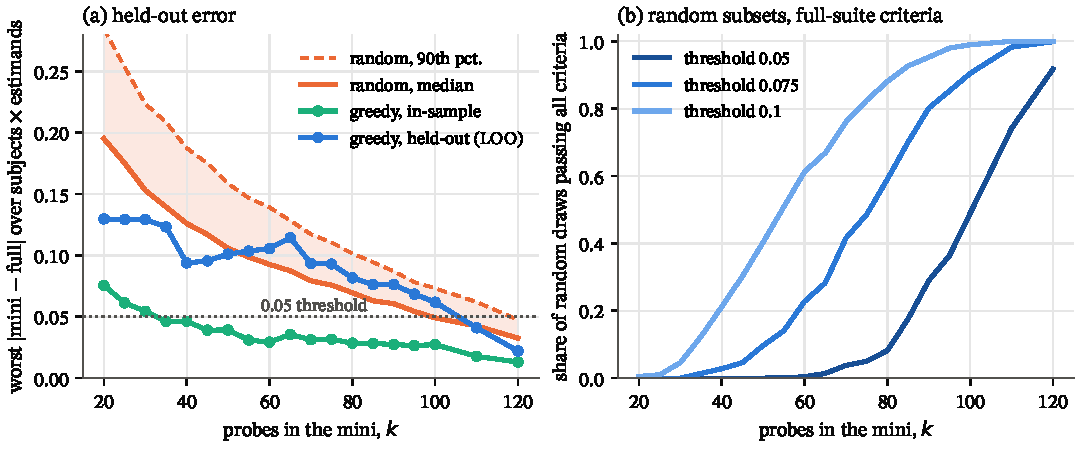
\includegraphics[width=\linewidth]{figures/fig_mini_k}
\caption{(a) Worst absolute error over subjects and estimands as a function
of mini size: greedy in-sample and held-out (leave-one-subject-out), and the
median and 90th percentile of 1000 random subsets. Greedy fits the training
subjects far below the 0.05 line while its held-out error rides the random
median until $k\ge110$. (b) Share of random subsets passing all criteria at
the preregistered 0.05 tolerance and at two looser ones (exploratory).}
\label{fig:k}
\end{figure}

\begin{table}[t]
\centering
\small
\caption{Preregistered grid, selected sizes. Worst held-out error is the
maximum over the twelve leave-one-subject-out folds and the defined estimands;
pass rates are over 1000 draws at the 0.05 criteria.}
\label{tab:grid}
\begin{tabular}{rccccc}
\toprule
$k$ & greedy in-sample & greedy held-out & pass & random pass & stratified pass \\
\midrule
40  & 0.046 & 0.094 & no  & 0.00 & 0.00 \\
60  & 0.029 & 0.106 & no  & 0.01 & 0.01 \\
70  & 0.031 & 0.093 & no  & 0.04 & 0.03 \\
80  & 0.028 & 0.082 & no  & 0.11 & 0.10 \\
100 & 0.027 & 0.062 & no  & 0.52 & 0.46 \\
110 & 0.018 & 0.041 & yes & 0.72 & 0.75 \\
120 & 0.013 & 0.022 & yes & 0.93 & 0.95 \\
\bottomrule
\end{tabular}
\end{table}

\subsection{The frozen mini at \texorpdfstring{$k=110$}{k=110}}

The greedy subset selected on all twelve subjects at $k=110$ contains 47
not-Islamic, 32 names-Islam and 31 intrinsic scenarios (bank shares 39/31/30
percent), covers every pillar, and is released as \texttt{mini\_v1.json}
against probe-bank v4. \Cref{tab:ladder} gives its validation ladder.
Held-out, its worst error is 0.041 (GLM-5.1's headline); in-sample 0.018. It
produces no sign flip and preserves every separated pair. Per judge it is
marginal: with Opus alone the held-out worst is 0.043, with Gemini alone
0.052 --- one cell, GLM-5.1's headline, two thousandths over. Both judges pass
in-sample. The mini should therefore be quoted as a pooled-judge number.

The two never-in-selection rungs pass comfortably. On the Arabic run (nine
subjects, including Claude Opus 4.8, which has no English run) the worst
error is 0.034, and the Arabic--English rank correlation on the eight shared
subjects is 0.833 on the full bench and 0.833 on the mini. On the four
follow-up variants the worst error is 0.024. Per-pressure steadfastness,
which was not gated, exceeds 0.05 in three of 72 cells (maximum 0.062: the
personal-appeal and false-authority cells of Ansari and GPT-5.5).

Bootstrap-over-scenarios confidence intervals on the mini are 4 to 9\% wider
than on the full bench, against $\sqrt{140/110}=1.13$ expected under
independence; the frozen subset is slightly more homogeneous than a random
one. Finally, the in-sample objective the greedy method optimizes can be
pushed further: annealing reaches 0.012 and the MILP an incumbent of 0.007
before its time limit, so greedy's in-sample gap is at least 0.011. None of
that is relevant held-out, as the next subsection shows.

\begin{table}[t]
\centering
\small
\caption{Validation ladder for the frozen 110-scenario mini. Worst absolute
error over subjects and defined estimands; E2 is satisfied on every rung.}
\label{tab:ladder}
\begin{tabular}{llcc}
\toprule
Rung & Data & Worst error & Pass at 0.05 \\
\midrule
In-sample fit (not headlined) & 12 subjects, selected on all & 0.018 & yes \\
V1 leave-one-subject-out & 12 folds & 0.041 & yes \\
V2 per judge, Opus 4.8 only & held-out & 0.043 & yes \\
V2 per judge, Gemini 3.1 Pro only & held-out & 0.052 & no \\
V3 Arabic replication & 9 subjects, never in selection & 0.034 & yes \\
Follow-up variants & 4 subjects, never in selection & 0.024 & yes \\
Per-pressure steadfastness (not gated) & 72 cells & 0.062 & 3 cells over \\
V4 prospective & K2-Horizon-375B, released after the freeze & 0.019 & yes \\
\bottomrule
\end{tabular}
\end{table}

\subsection{Why 110: the sampling floor}\label{sec:floor}

This subsection is exploratory in the sense that it was computed after the
grid, but it involves no fitting and could have been done first. For a
subject, let $\sigma$ be the standard deviation across the 140 scenarios of
the per-scenario mean band on the reported scale. Across the twelve subjects
$\sigma$ runs from 0.32 (Fanar-Sadiq) to 0.62 (GPT-5.5), median 0.53. A
random subset of $k$ scenarios then estimates the headline with a
finite-population standard error of
\[
\text{SE}(k)=\sigma\sqrt{\tfrac{1}{k}-\tfrac{1}{140}},
\]
which for the median subject is 0.070 at $k=40$, 0.044 at 70, 0.028 at 100,
0.023 at 110 and 0.018 at 120. The criteria demand that the worst of roughly
44 held-out cells (twelve subjects, four estimands, a few undefined) stay
under 0.05. The expected maximum of 44 roughly normal errors is about 2.2
standard errors, so the requirement is SE $\lesssim0.02$, i.e.\ $k\gtrsim110$.
The random pass-rate curve in \cref{fig:k}(b) is this arithmetic made
empirical.

The point is that a selection method can only beat this floor if the
scenario-level structure it exploits transfers to a subject it has not seen.
The in-sample/held-out gap says it does not: what greedy learns from eleven
subjects is largely which scenarios happen to balance \emph{those} subjects'
errors, and a twelfth subject --- especially an outlier like Ansari --- has
its own. Annealing and the MILP learn more of the same, which is why their
in-sample gains do not appear held-out.

\subsection{Sensitivity to the criteria (exploratory)}

Because the tolerance and the estimand set were fixed in advance, it is fair
to ask what they cost. Re-scoring the stored leave-one-subject-out folds under
looser criteria: at a 0.075 tolerance the full suite passes from $k=95$ (a
32\% saving) and the headline alone from $k=35$; at 0.10, from $k=40$ and
$k=20$. Random draws pass the full suite at 0.075 in 59\% of cases at $k=80$
and 91\% at $k=100$. So the pilot's optimistic picture was not wrong about
the headline at a loose tolerance; it was wrong about what a mini must
reproduce and how tightly. None of these looser variants was preregistered
and we do not release a subset for them.

\subsection{Prospective test}\label{sec:v4}

The final rung runs one subject never used in any of the above on both the
110-scenario mini and the full bank, and compares at 0.05. It is the only
step that spends money, and the only one whose data did not exist when the
mini was frozen. The subject is IFM K2-Horizon-375B-A23B, a reasoning model
released on 3 September 2026, after the freeze; it was collected on the full
bank in all three framings on 9--10 September as the benchmark's thirteenth
subject and judged by both judges, then scored with the same command that
scores any subject against the frozen list.

The mini reproduces every estimand inside the preregistered bound. Headline:
$-0.438$ on the mini against $-0.448$ on the full bank (error 0.011).
Steadfastness: $-0.097$ against $-0.088$ (0.009). Faith stated: $-0.049$
against $-0.068$ (0.019). Guided: $+0.521$ against $+0.510$ (0.011). The
worst error, 0.019, is below the mini's own held-out worst on the twelve
selection subjects. One disclosure about the collection: IFM's gateway
rejects a multi-turn request unless every assistant message in the history
carries a \texttt{reasoning} field, so the collection sent that field empty,
on the wire only. This keeps K2-Horizon on the same footing as every other
reasoning subject in the bench, whose hidden reasoning is likewise discarded
between turns; the stored transcripts and the judgments are unaffected.

\section{Discussion}\label{sec:discussion}

The result is a negative one for optimized item selection on this benchmark
and, we think, on benchmarks of its shape. The item-reduction successes in
the literature share features JaleesBench lacks: thousands of items, so that
a hundred selected ones is a two-orders-of-magnitude saving rather than a
21\% one; hundreds of models or model--prompt pairs to fit item parameters
on, rather than twelve subjects; and a single accuracy to reproduce, often
only its ranking. With twelve subjects there is not enough cross-subject
signal to learn which scenarios are ``anchors,'' and with four estimands per
subject the worst-cell criterion is unforgiving. Under those conditions the
floor is the sampling floor, and the only lever is $k$.

Two practical conclusions follow. First, compute $\sigma\sqrt{1/k-1/N}$
against the tolerance and the number of gated cells before writing a
selector; if the answer is close to $N$, the study is a sampling study, not a
selection study. Second, when a selector is used, report it held-out with
the in-sample number beside it, because the gap between the two is the
evidence of overfitting and is the more informative quantity.

The mini itself is fit for its stated purpose: cheap screening and tracking
of a subject across versions, at a fifth off the cost, with errors below
0.05 on every reported quantity for every subject we can test. It should not
be cited in place of the full bench, it should be quoted pooled over judges,
and it is versioned against probe-bank v4; any change to the bank re-runs
selection.

\section{Limitations}\label{sec:limitations}

Twelve subjects is a small population to validate on, and one of them
(Ansari) dominates the held-out failures; a thirteenth outlier in the other
direction could fail the mini at 110. The per-judge rung fails by 0.002 for
one judge, which we report rather than round away. The 0.05 tolerance is a
choice, and \cref{sec:results} shows how much it costs. The prospective test
is a single subject, and one that sits in the crowded lower half of the
scale. And the selection methods compared are the ones fixed in
advance; a method that borrows strength across subjects with an explicit
item model might do better with more subjects, though \cref{sec:floor}
bounds how much better on this bank.

\section{Availability}\label{sec:availability}

The selection and validation code, the frozen scenario list, every number in
this paper, and the tests that check the full-bench references against the
published JaleesBench statistics are in the JaleesBench repository
(\texttt{jaleesbench/mini.py}, \texttt{data/mini\_v1.json},
\texttt{results/mini\_stats.json}). A single command reproduces the study
from the judgment files with the fixed seed.

\bibliographystyle{plainnat}
\bibliography{references}

\end{document}
